\documentclass[Master, ngerman, UKenglish]{scrbook}
%------------------------------------------------------------------------------
% This file contains a skeleton thesis for
% a Physics or Astronomy Institute in the University of Bonn

% Specify the thesis type as an option: PhD, Master, Diplom, Bachelor
% Specify the thesis stage as an option: Draft (default), Submit, Final, PILibrary

% Specify the language(s) in the class and then use babel.
% If you need more than one language, give the default language last,
% e.g. ngerman, UKenglish for a thesis in British (UK) English where you want
% to be able to set the language to German for some part of it.

%------------------------------------------------------------------------------
% Pass TeX Live version to the package
% Use command pdflatex --version to find out which version you are running
% Add option backref=false when your thesis is ready to turn off back-referencing
% in your bibliography
\usepackage[texlive=2020]{ubonn-thesis}
% Adjustments to standard biblatex style
\usepackage{ubonn-biblatex}

% Glossary package
% \usepackage[acronym,toc,nosuper]{glossaries}
\usepackage{acro,hyperref,longtable,tabu}
% TikZ packages and libraries
% \usepackage{tikz}
% \usepackage{tikz-3dplot}
% \usepackage{pgfplots}
% \usetikzlibrary{positioning,shapes,arrows}
% \usetikzlibrary{decorations.pathmorphing}
% \usetikzlibrary{decorations.markings}
\usepackage{thesis_defs}
\usepackage{multirow}
\usepackage{physics}

%------------------------------------------------------------------------------
% Instead of colouring  links, cites, table of contents etc.
% put them in a coloured box for the screen version.
% This is probably a good idea when you print your thesis.
% \hypersetup{colorlinks=false,
%   linkbordercolor=blue,citebordercolor=magenta,urlbordercolor=darkgreen
% }

%------------------------------------------------------------------------------
% When writing your thesis it is often helpful to have the date and
% time in the output file. Comment this out for the final version.
\ifoot[\today{} \thistime]{\today{} \thistime}

% In order to check if your labels are referenced try the refcheck package
% \usepackage{refcheck}

%------------------------------------------------------------------------------
% biblatex is included by ubonn-thesis. Look there for the settings used.
% See the options for settings that can be changed easily.
% For further changes copy the \RequirePackage[...]{biblatex} here
% and include ubonn-thesis with the option biblatex=false.

% Specify the bibliography files here and not at the end!
% Use standard_refs-bibtex if you use bibtex or bibtex8
% and standard_refs-biber  if you use biber
\addbibresource{bib/thesis_refs.bib}
%\addbibresource{bib/standard_refs-biber.bib}

%------------------------------------------------------------------------------
% The following definitions are used to produce the title pages
% needed at various stages
\newcommand{\thesistitle}{Raman manipulation between momentum state components of ultracold erbium atoms}
\newcommand*{\thesisauthor}{Pedro Castro Perez}
\newcommand*{\thesistown}{Tremp (LLeida), Spain}
\renewcommand*{\InstituteName}{\IAP}
\renewcommand*{\inInstitute}{\inIAP}
\renewcommand*{\InstituteAddress}{\IAPaddress}
% Adjust \thesisreferee...text depending on male/female referee
\newcommand*{\thesisrefereeonetext}{1.\ Gutachter}
\newcommand*{\thesisrefereeone}{Prof.\ Dr.\ Martin Weitz}
\newcommand*{\thesisrefereetwotext}{2.\ Gutachter}
\newcommand*{\thesisrefereetwo}{Prof.\ Dr.\ }
% Date when thesis was submitted (Master/Diplom)
% Year or Month, Year when thesis was submitted (PhD)
\newcommand*{\thesissubmit}{01.06.2021}
% \newcommand*{\thesissubmit}{Month 2020}
% Date of thesis examination (PhD)
\newcommand*{\thesispromotion}{XX.YY.2021}
% Month and year of the final printed version of the thesis
\newcommand*{\thesismonth}{Juni}
\newcommand*{\thesisyear}{2021}
\newcommand*{\thesisnumber}{BONN-IR-2021-XXX}

%------------------------------------------------------------------------------
% The abstract is only needed for the printed version and should be in
% English regardless of the language of the thesis
\newcommand{\thesisabstract}{%
  \begin{otherlanguage}{UKenglish}
    This is your thesis abstract. It may be in a language that is
    different from the rest of your thesis.
  \end{otherlanguage}
}

%------------------------------------------------------------------------------
% \includeonly can be used to select which chapters you want to process
% A simple \include command just inserts a \clearpage before and after the file
% Note that \includeonly can be quite picky! Do not forget to put a
% comma after the filename, otherwise it will simply be ignored!
 \includeonly{%
   1_thesis_intro,
   2_thesis_bec_condensation,
   3_thesis_bec_diffraction,
   4_thesis_raman_manipulation,
   5_thesis_results,
   thesis_appendix,
   thesis_acknowledge
 }

%------------------------------------------------------------------------------
% Give a list of directories where figures can be found. Do not leave
% any spaces in the list and end the directory name with a /
\graphicspath{%
  {figs/}%
  {figs/cover/}%
}

%------------------------------------------------------------------------------
% Make a list of acronyms
\acsetup{list/template=longtabu, list/heading=addchap}

\DeclareAcronym{bec}{short=BEC,long=Bose-Einstein condensate}
\DeclareAcronym{mot}{short=MOT,long=magneto-optical trap}
\DeclareAcronym{odt}{short=ODT,long=optical dipole trap}
\DeclareAcronym{ai}{short=AI,long=absorption imaging}
\DeclareAcronym{tc}{short=TC,long=transversal cooling}
\DeclareAcronym{zs}{short=ZS,long=zeeman slower}
\DeclareAcronym{ule}{short=ULE cavity,long=ultra low expansion cavity}
\DeclareAcronym{aom}{short=AOM,long=acousto-optic modulator}
\DeclareAcronym{ec}{short=EC,long=effusion cell}
\DeclareAcronym{hl}{short=HL,long=hot lip}
\DeclareAcronym{uhv}{short=UHV,long=ultra-high vacuum}
\DeclareAcronym{dfc}{short=DFC,long=dual filament effusion cell}
\DeclareAcronym{rms}{short=RMS,long=root mean squared}
\DeclareAcronym{quest}{short = QUEST, long = Quasi-electrostatic trap}
\DeclareAcronym{tof}{short = TOF, long = time of flight}
\DeclareAcronym{pbs}{short = PBS, long = polarization beam spliter}
\DeclareAcronym{rf}{short = RF, long = radio frequency}


% Draft version - add the word DRAFT on the cover pages
\ifthenelse{\equal{\ThesisVersion}{Draft}}{%
  \usepackage{background}
  \ifthenelse{\texlive < 2013}{%
    \SetBgContents{DRAFT}
    \SetBgColor{blue!30}
  }{%
    \backgroundsetup{contents=DRAFT, color=blue!30}
  }
}

%------------------------------------------------------------------------------
\begin{document}

% Cover page of thesis - this is only needed for the printed final
% version to be submitted to the department library
% Do not use this page for thesis submission to the Prüfungsamt or Promotionsbüro!
\ifthenelse{\equal{\ThesisVersion}{PILibrary}}{%
  \typeout{Document \jobname, Info: PI library version of thesis}
  \input{../Template/cover/\ThesisType_Cover}
}{}

% Start counting pages from the title page
\frontmatter
% Dedication has to come before \maketitle
% \dedication{Dedicated to no one}

% Select the correct title page(s)
\ifthenelse{\equal{\ThesisType}{Unknown}}{%
  \typeout{Document \jobname, Error: Unknown thesis type - no title page printed}
}{%
  % Bachelor thesis only has one title page
  \ifthenelse{\equal{\ThesisType}{Bachelor}}{%
    \typeout{Document \jobname, Info: Bachelor thesis}
    \input{../Template/cover/\ThesisType_Title}
  }{%
    \ifthenelse{\equal{\ThesisVersion}{Final} \OR \equal{\ThesisVersion}{PILibrary}}{%
      % Final and PI library versions
      \typeout{Document \jobname, Info: Final version of a \ThesisType  thesis}
      \input{../Template/cover/\ThesisType_Final_Title}
    }{% Submission and draft versions
      \input{../Template/cover/\ThesisType_Submit_Title}
      \typeout{Document \jobname, Info: Draft/submission version of a \ThesisType  thesis}
    }
  }
}

\pagestyle{scrplain}

%------------------------------------------------------------------------------
% You can add your acknowledgements here - don't forget to also add
% them to \includeonly above
%------------------------------------------------------------------------------
\chapter*{Acknowledgements}
\label{sec:ack}
%------------------------------------------------------------------------------


%%% Local Variables: 
%%% mode: latex
%%% TeX-master: "../Template/Thesis"
%%% End: 


\tableofcontents

\mainmatter
\pagestyle{scrheadings}

% Turn off DRAFT for the following pages
\ifthenelse{\equal{\ThesisVersion}{Draft}}{%
  \ifthenelse{\texlive < 2013}{%
    \SetBgContents{}
  }{%
    \backgroundsetup{contents={}}
  }
}{}

%------------------------------------------------------------------------------
% Add your chapters here - don't forget to also add them to \includeonly above
% !TEX root = Thesis.tex

%==============================================================================
\chapter{Introduction}
\label{chap:intro}
%==============================================================================

The first theorization of an ultracold ensemble of atoms was performed by Satyendra Nath Bose and Albert Einstein in 1924 during a series of publications where the concept of what is today known as a \acf{bec} was developed \cite{Bose1924, Einstein1924, Einstein1925}. At the time, this was a new state of matter formed by bosonic particles occupying the energetic ground state macroscopically for close to absolute zero temperatures. It took more than 70 years to obtain this theorized state of matter in an experiment. The first \acp{bec} were generated in 1995 by several research groups for three different chemical elements: rubidium \cite{Davis1995}, sodium \cite{Anderson1995} and lithium \cite{Bradley1995}. The following years lead to a rising interest of this exotic state of matter due to their quantum properties that allow to describe the system of particles by using just the coherent wave function of a single-particle. Due to this, \acp{bec} for many other elements were achieved. Some examples are: alkali metals like strontium \cite{Stellmer2009}, and Lanthanides like ytterbium \cite{Takasu2003}, dysprosium \cite{Lu2011} and erbium \cite{Aikawa2012}. Even in non-atomic bosonic particles like photons \cite{Klaers2010}.

Nowadays, there has been increasing interest in the condensation of atoms belonging to the lanthanide group. This is due to two main reasons: the first one being the large magnetic moment that these elements normally have, which increases the effect of dipole-dipole interaction \cite{Aikawa2012,Baier2018}. The second reason will be more relevant for this experiment and is based on the fact that these atoms normally have a non-vanishing electronic angular momentum in their energetic ground state. For the case of erbium, the orbital angular momentum has a value of $L=5$ for the ground state. This allows to use Raman transitions between Zeeman sublevels of the ground state in the fine structure scheme. Increasing the available detuning ranges, which enables the possibility of using large values for the detuning. This reduces the photon scattering rates and increases the coherence times for the \ac{bec} \cite{Grimm2000}.

Raman manipulation permits the use of a method called phase imprinting, which generates synthetic magnetic fields and have been theorised to be achievable with lanthanide atoms \cite{cui2013synthetic}. If these synthetic fields were generated with enough strength, it would enable the fractional quantum Hall regime for neutral atoms. This could have major implications possibly enabling studies of topological quantum computation. The synthetic magnetic fields have already been observed as vortices structures inside the \ac{bec} for rubidium \cite{Lin2009}. However, the strength of these fields was limited by the coherence time of the available transitions in this element. As said, the use of erbium permits longer coherence times, which could generate larger synthetic magnetic fields and possibly enable the fractional quantum Hall regime. In order to achieve the Raman manipulation process required, the starting point for this work will be the generation of an erbium (Er$^\text{168}$) \acf{bec} with an approximate atom number of 50000.

This thesis aims to study a Raman manipulation set-up formed by two counter-propagating beams detuned with respect to an erbium transition near \SI{841}{\nano\meter}. The main part will consists of the characterisation of Raman transitions between momentum states for the energetic ground state of erbium. This corresponds to the atomic \ac{bec} diffraction with the Raman beams forming and optical lattice. The resulting effect is the generation of different momentum orders, similar to the well-known process of light diffraction. After this, the main focus will be on the achievement of Raman transitions into the spin-momentum configuration between different sublevels, generated by Zeeman splitting of the ground energy level of the erbium \ac{bec}. This achievement represents the ground work for the future realisation of strong enough synthetic fields to reach the fractional quantum Hall regime. However, in order to obtain the Raman manipulation of internal spin states, an additional experiment with \ac{rf} transitions is required. Its main purpose is to characterise and prepare the magnetic fields causing the Zeeman splitting of the ground state.

Therefore, the thesis it is divided in different chapters according to its content. Chapter \ref{chap:erbium_bec} shows the properties of erbium, introduces the basic theory of an atomic \ac{bec} and briefly describes the experimental set-up used to achieve and measure an erbium \ac{bec}. Chapter \ref{chap:one_dimensional_lattices} gives the theoretical basis for the diffraction of a \ac{bec} with an optical lattice. Chapter \ref{chap:raman_manipulation} describes the \ac{rf} transitions experiment together with a basis of the Raman manipulation of the spin-momentum space. Chapter \ref{chap:results_and_discussion} shows the measured and analysed results. And finally, \ref{chap:outlook} serves as a conclusion and outlook to the thesis.

%%% Local Variables: 
%%% mode: latex
%%% TeX-master: "Thesis"
%%% End: 

% !TEX root = Thesis.tex

%==============================================================================
\chapter{Erbium \acl*{bec}}
\label{chap:erbium_bec}
%==============================================================================

This chapter has the objective of briefly review some relevant properties of Erbium, which will clarify what makes it relevant in the study of ultracold atoms. After this, the basic theory of Bose-Einstein condensation will be discussed, along with a brief description of the experimental phases required to create and observe an erbium \ac{bec}. This experimental realisation will be the foundation on which the following chapters will be grounded when discussing further experimental achievements.

%==============================================================================
\section{Properties of erbium} \label{sec:erbium_properties}
%==============================================================================
Erbium is a chemical element with an atomic number of 68, which belongs to the series of Lanthanides. It is also part of the group called rare-earth elements and it was first discovered by G. Monsander in 1843 \cite{mosander1843xxx}. The name of ``Erbium'' comes from the name of the Swedish village of Ytterby, the place where it was extracted. At that time, the similarity of rare-earth metals' chemical properties made their distinction extremely difficult. For this reason, what G. Monsander thought to be pure Erbium oxide was in fact a mixture of different rare-earth metal oxides. The element is not obtained in a reasonably pure form until 1937 by W. Klemm and H. Bommer \cite{klemm1937bommer}.

Considering some basic properties of this element, under standard conditions erbium is in a solid state. It has a silver shining surface, which oxidises with air contact. This rare-earth metal has a melting point of \SI{1802}{\kelvin} and boiling point of \SI{3136}{\kelvin}. As a result, to be able to work with a free atomic gas of erbium requires to heat up the solid metal of erbium to high temperatures \cite{emsley1998}.

The number of stables erbium isotopes is 6 , which are given in Table \ref{tab:Isotopes_Erbium}. All of them are bosons with nuclear spin of zero, in exception of $^{\text{167}}\text{Er}$, which is a fermion with nuclear spin of 7/2. The chosen isotope for this experiment is $^{\text{168}}\text{Er}$ because of its bosonic nature (see Section \ref{sec:bose-einstein_condensation}), high abundance and favourable scattering properties \cite{Frisch2014}.

\begin{table}[htbp] \centering
	\begin{tabular}{@{}c|c|c|c@{}}\hline
		Isotope                  & Abundance [\%]          & Atomic Mass [u] & Nuclear Spin [$\hbar$] \\ \hline\hline
		$\text{Er}^{\text{162}}$ &  0.14                   & 161.928775      & 0   \\
		$\text{Er}^{\text{164}}$ &  1.61                   & 163.929198      & 0   \\ 
		$\text{Er}^{\text{166}}$ & 33.60                   & 165.930290      & 0   \\
		$\text{Er}^{\text{167}}$ & 22.95                   & 166.932046      & 7/2   \\
		$\text{Er}^{\text{168}}$ & 26.80                   & 167.932368      & 0   \\  
		$\text{Er}^{\text{170}}$ & 14.90                   & 169.935461      & 0   \\  \hline
	\end{tabular}
	\caption[Table with the stable isotopes of Erbium]{Table with the stable isotopes of Erbium that can be found on Nature with their respective Abundance ratio, Atomic mass and Nuclear Spin. Spectroscopy data taken from \cite{sansonetti2005handbook}.}\label{tab:Isotopes_Erbium}
\end{table}

In addition to these properties, erbium atoms have a rather complex energetic level scheme due to its open 4f shell. This one lacks 2 electrons to be completely filled, which makes erbium to have an electronic ground state with an orbital angular momentum value of $L = 5$ and a magnetic moment of seven Bohr magneton $7\mu_B$ \cite{ban2005laser}. This high value for the orbital angular momentum in the ground state of erbium provides several advantages for Raman-coupling processes. Leading to longer coherence times and stronger synthetic magnetic fields when comparing with alkali metals like rubidium or caesium, commonly used in ultracold atoms experiments  \cite{cui2013synthetic}.


A scheme of erbium energy levels together with the atomic transitions used in this experiment can be seen in figure \ref{fig:erbium_scheme}. The scheme shows that the electronic ground state of erbium is $\text{[Xe] }\text{4f}^{12} \text{6s}^2$, where [Xe]
represents the complete electronic configuration of Xenon\footnote{$\text{[Xe] = }\text{1s}^2 \text{ 2s}^2 \text{ 2p}^6 \text{ 3s}^2 \text{ 3p}^6 \text{ 3d}^{10} \text{ 4s}^2 \text{ 4p}^6 \text{ 4d}^{10} \text{ 5s}^2 \text{ 5p}^6$}. Moreover, the used optical transitions are represented by coloured arrows in the figure and its spectroscopic data is shown in table \ref{tab:Transitions}. From now on, these three transitions will respectively be referred to as the 401nm, 583nm, and 841nm transitions.

Finally, it must be noted that aside from the discussed application in ultracold atoms, erbium is used in multiple commercial applications. One prominent example is the use or erbium as a fibre amplifier in doped silicon fibers \cite{mears1987low}. Furthermore, in nuclear physics it is used as neutron absorbing control rods \cite{emsley2011nature}.

%\sisetup{per-mode = symbol}%

\begin{table}[htbp] \centering
	\begin{tabular}{@{}l|c|c|S|S|S@{}}\hline
		\multicolumn{3}{c|}{Parameters} & \multicolumn{3}{c}{Transitions} \\ \hline
		Name & Symbol & Unit & \multicolumn{1}{c|}{401nm} & \multicolumn{1}{c|}{583nm} & \multicolumn{1}{c}{841nm} \\ \hline\hline
		Wavelength in vacuum & $\lambda$	& \si{\nano\meter}					& 400.91		& 582.84		& 841.22\\
		Lifetime 			& $\tau$	& \si{\micro\second}				& 0.045			& 0.857			& 20   \\ 
		Natural linewidth 	& $\Delta \nu_0$	& \si{\kilo\hertz}					& \num{33370} 	& 185.71 		& 7.96   \\
		Decay rate 			& $\Gamma$	& \si{\per\second}					& \num{2.22e8} 	& \num{1.17e6}  & \num{5.00e4} \\
		Saturation intensity & $I_{S}$	& \si{\milli\watt\per\centi\meter}	& 71.80			& 0.12			& 0.00172  \\  
		Doppler temperature	& $T_D$	& \si{\micro\kelvin} 				& 848.69  		& 4.46  		& 0.19    \\  
		Doppler velocity	& $v_D$	& \si{\centi\meter\per\second}		& 21.5 			& 1.49 			& 0.31 \\
		Recoil temperature	& $T_R$	& \si{\nano\kelvin} 				& 354.95  		& 167.94  		& 80.43    \\  
		Recoil velocity	& $v_R$	& \si{\milli\meter\per\second}		& 5.93 			& 4.08 			& 2.82 \\  \hline
	\end{tabular}
	\caption[Spectroscopic data for the optical transitions of Erbium]{Spectroscopic data for the optical transitions of Erbium used in this experiment. These transitions are called the 401nm, 583nm, and 841nm transitions and can be seen in figure \ref{fig:erbium_scheme}. Shown spectroscopic data taken from \cite{mcclelland2006natural, lawler2010atomic, den2010radiative, ban2005laser, lipert1993isotope}}\label{tab:Transitions}
\end{table}


\pagebreak


\begin{figure}[!htbp]\centering
	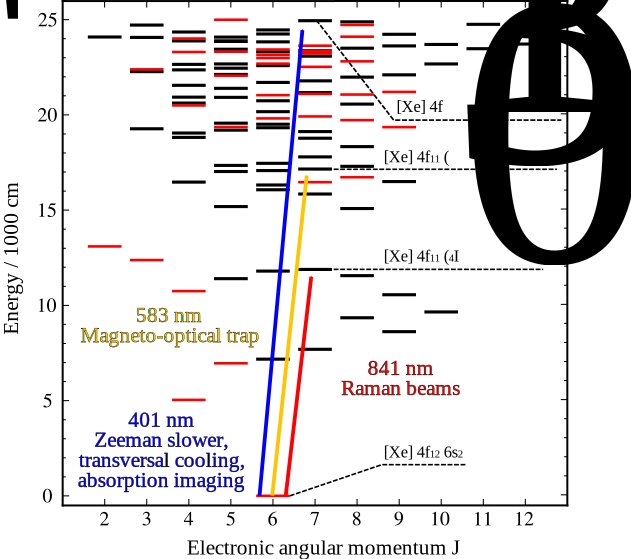
\includegraphics[width=1.\columnwidth]{erbium_term_scheme.pdf}
	\caption[Erbium energy scheme]{Energy level scheme of Erbium represented as a function of the total angular momentum J. This scheme shows only a range of energies relevant for the experiment of up to 25000 $\text{cm}^{\text{-1}}$. The different arrows show the used transitions and for which phase of the experiment they are used for. The red lines represent energy states with even parity and the black lines those with odd parity. Data taken from \cite{NIST}. }\label{fig:erbium_scheme}
\end{figure}


%==============================================================================
\section{Bose-Einstein Condensation} \label{sec:bose-einstein_condensation}
%==============================================================================

A \ac{bec} is generally defined as a state of matter formed when a gas of bosons with a low density is cooled to near-zero temperatures (typically a few hundreds \si{\nano\kelvin}). To understand this definition and the next theoretical principles, it is necessary to explain what is a Boson. In quantum mechanics, bosons are defined as particles with an integer value in their spin. This characteristic makes them have a symmetric wave function under the interchange of two particles, which allows multiple bosons in a given system to be in the same quantum state. Unlike the counterpart fermions, particles counting with a half odd integer spin and an anti-symmetric wave function. This case leads to Pauli's exclusion principle that avoids more than one fermion to occupy the same quantum state \cite{Pauli1925}.

It was the Indian physicist S. N. Bose in 1924, the first one who described in a successful way an ideal gas of non interacting free photons, behaving like mass-less bosons. His idea was initially rejected for publication in scientific journals. However, Bose sent the manuscript to A. Einstein, who recognized its importance, translated the paper to German and saw to it that was published \cite{Bose1924}. After this, Einstein extended Bose's treatment to massive particles and predicted the occurrence of a phase transition in a gas of non-interacting atoms, what is today known as a \ac{bec} \cite{Einstein1924, Einstein1925}.

These publications led to Bose-Einstein statistics, a model that explains the energetic behaviour of a non-interacting gas of indistinguishable $N$ bosons, each one with mass $M$ \cite{Masahito2010, Pethick2008}. The average number of particles at a given non-degenerate state with wave vector $\mathbf{k}$ and energy $E_\mathbf{k} = \hbar^2 \mathbf{k}^2 / 2M$ is given by

\begin{equation}\label{eq:bose-einstein_distribution}
	\bar{N}_{\mathbf{k}} = \frac{1}{e^{(E_\mathbf{k} - \mu)/k_B T} - 1},
\end{equation}
for an ideal gas of bosons in thermal equilibrium at a temperature $T$, Boltzmann constant $k_B$ and chemical potential $\mu$, which depends of $N$ and $T$ \cite{Masahito2010}. The total number of particles in all energy states is expressed as

\begin{equation}\label{eq:chemical_potential_relation}
N = \sum_{\mathbf{k}}\frac{1}{e^{(E_\mathbf{k} - \mu)/k_B T} - 1}.
\end{equation}

So the chemical potential $\mu$ is determined such that Eq. \eqref{eq:chemical_potential_relation} is satisfied for any given $N$ remaining constant. Now, expanding into the thermodynamic limit where $N$ and the occupied volume $V$ are increased to infinite values keeping the particle density $n = V/N$ constant. The sum over $\mathbf{k}$ appearing in Eq. \eqref{eq:chemical_potential_relation} can be replaced by an integral such as

\begin{equation}\label{eq:thermodynamic_limit}
n = \frac{N}{V} =  \frac{1}{(2\pi)^3}\int d^3 k\frac{1}{e^{(E_\mathbf{k} - \mu)/k_B T} - 1}.
\end{equation}

For decreasing values of $T$ and constant $n$, the chemical potential increases becoming zero at a critical temperature $T_C$. By making $\mu = 0$, $T = T_C$ and $E_\mathbf{k} = \hbar^2 \mathbf{k}^2 / 2M$ in Eq. \eqref{eq:thermodynamic_limit} results

\begin{equation}\label{eq:thermodynamic_limit_at_critical_conditions}
n =  \zeta(3/2) \bigg(\frac{M k_B T_C}{2 \pi \hbar^2}\bigg)^{3/2},
\end{equation}
where $\zeta(3/2) \simeq 2.612$ denotes the Riemann zeta function evaluated at 3/2. So the critical temperature of the \ac{bec} is given by

\begin{equation}\label{eq:critical_temperature}
T_C = 3.31 \frac{\hbar^2 n^{2/3}}{k_B M}.
\end{equation}

A relevant case of study is when $T < T_C$ because a fraction of the $N$ bosons remains in the ground state with an energy $E = 0$. So the ideal gas of bosons can be divided in two energetic groups $N = N_{E=0} + N_{E>0}$. It must be noted that, the replacement of a sum by an integral in Eq. \eqref{eq:thermodynamic_limit} can only be take place in group of particles with an energy greater than zero $E>0$. As a result of this, the integral of Eq. \eqref{eq:thermodynamic_limit} for the case $T < T_C$ results

\begin{equation}\label{eq:thermodynamic_limit_low_T}
\frac{N_{E>0}}{V} = \zeta(3/2) \bigg(\frac{M k_B T}{2 \pi \hbar^2}\bigg)^{3/2}.
\end{equation}

Using now equations \eqref{eq:critical_temperature}, \eqref{eq:thermodynamic_limit_at_critical_conditions} and the fact that $N_{E>0} = N - N_{E=0}$ results in an expression of the relative population of a \ac{bec} in an ideal bosons gas as a function of temperature:

\begin{equation}\label{eq:bec_relative_population}
\frac{N_{E=0}}{N} = 1 - \bigg(\frac{T}{T_C}\bigg)^{3/2}.
\end{equation}

An intuitive way to think about this is to imagine the bosons as wave packets with a size of the thermal de Broglie length $\lambda_{th}$. This parameter is conventionally defined \cite{deBroglie1970}.

\begin{equation}\label{eq:de_Broglie_length}
\lambda_{th} = \frac{h}{\sqrt{2\pi Mk_B T}}.
\end{equation}

For falling temperatures, the thermal de Broglie length begins to increase and the wave packets representing the bosons become greater in size. At $T\lesssim T_C$ the particles begin to occupy macroscopically the ground state and its wave packets start to overlap forming a macroscopic wave function, capable of describing the whole particle system. This is one of the most relevant properties of a \ac{bec}. Now, we combine equations \ref{eq:thermodynamic_limit_at_critical_conditions} and \ref{eq:de_Broglie_length} to obtain for a squared well potential the critical value

\begin{equation}\label{eq:phase_space_critical_point}
\qquad\qquad\qquad n \lambda_{th}^3 = \zeta(3/2) \simeq 2.612 \qquad \textrm{for } \ T=T_C.
\end{equation}

This product of density with cubic de Broglie length is defined in the literature as phase-space density $\rho_{psd} \equiv n \lambda_{th}^3$. It is normally used as a parameter that helps to quantify any given bosonic system. From Eq. \eqref{eq:phase_space_critical_point}, one can deduce that to form a \ac{bec} with an atomic (bosonic) cloud in three dimensions the phase space density must fulfil $\rho_{psd} \geq 2.612$. As a result, the required conditions to form a \ac{bec} can only be fulfilled when the atomic cloud is sufficiently cold and dense. For the case of a three dimensional gas of atoms trapped in an harmonic potential this condition over the phase space density decreases to $\rho_{psd} \geq 1.2$ \cite{Pethick2008}. 

A further description about the theory of Bose-Einstein Condensation can be found in \cite{Masahito2010, Pethick2008}.

%==============================================================================
\section{Experimental realization of an erbium \ac{bec}} \label{sec:experimental_preparation}
%==============================================================================

The generation of an erbium \ac{bec} requires a multiple set of experimental phases, with each one based on different physical principles. The main purpose of this section is to discuss briefly every one of those together with its underlying foundation. For a more detailed description of the experimental set refer to  \cite{Ulitzsch2016}. 

Figure \ref{fig:table_set_up} shows a scheme of the experimental setup. It must be noted that all the devices used for the experiment lay on top of three optical tables represented in the figure by grey areas. Moreover, the laser beams produced by different laser systems are represented by coloured lines. The erbium atoms are at all times kept inside an \ac{uhv} system formed by an oven, \ac{zs} and main chamber. This \ac{uhv} is maintained by two ion getter pumps reaching a pressure of \SI{e-8}{\milli\bar}. Additionally, for the main chamber there is a titanium sublimation pump, which reduces the vacuum even further to \SI{e-10}{\milli\bar}. The need of an \ac{uhv} comes from the fact that to reach an atomic \ac{bec}, the cooling process must be so extreme that any interaction with room temperature atoms would lead to heating and destruction of the cold erbium cloud.


\begin{figure}[!htbp]\centering
	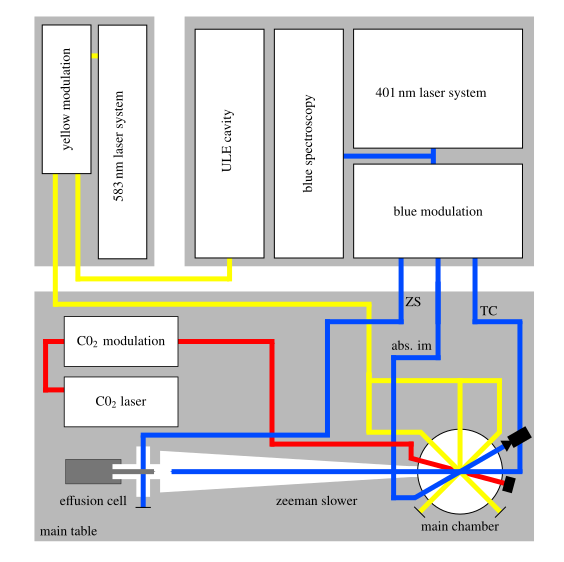
\includegraphics[width=1.\columnwidth]{table_set_up.pdf}
	\caption[Scheme of the experimental setup]{Scheme of the experimental setup. It is divided in three optical tables represented by grey areas. The 401nm laser system is used for the \acf{tc}, \acf{zs} and \acf{ai}. It is generated by a frequency doubled diode laser locked to a spectroscopic signal of the 401nm transition of $^{\text{168}}\text{Er}$. The 583nm laser system is used for the \acf{mot} and is frequency looked to an \acf{ule}. This trap uses 401nm laser beam in three spacial dimensions x, y and z. The $\text{CO}_{2}$ laser is used as main source of an \acf{odt}. The 841nm laser system is used to form the two lattice beams used for Raman transition processes which will be described in Chapters \ref{chap:one_dimensional_lattices} and \ref{chap:raman_manipulation}.}\label{fig:table_set_up}. 
\end{figure}

Most of the laser systems in this experiment produce resonant light for the $^{\text{168}}\text{Er}$ atomic transitions. For this reason, these light sources are kept on different optical tables separated from the \ac{uhv} system. Thus, unwanted atom-light interaction that could damage the cooling capabilities of the experiment is reduced. This laser light is guided into the main table by using optical fibres that can be blocked and unblocked through the use of mechanical shutters and \acp{aom} before the fibre coupler. Allowing for a fast response time (typically a few hundreds nanoseconds) and better control of the experimental phases.

The different phases required to obtain an erbium \ac{bec} are chronologically very organized. There is almost no temporal overlay between phases. This allows for a very accurate description of the experiment by just explaining every procedure in a chronological order. In every cycle, the atoms start in the oven and pass through the \ac{tc} and \acf{zs} to reach the main chamber, where the \ac{mot}, \ac{odt} and evaporative cooling take place to generate the erbium \acl*{bec}.

\subsection{Oven}\label{subsec:oven}

The required first step to form an erbium \ac{bec} consist in transforming a solid state metal, with a high purity of erbium atoms (typically over 99\%), into an atomic beam. The main reason for this is the fact that erbium is required to be in a gas state with very low interactions between each atom. In order to produce an erbium beam, an oven of the type known as \Acf{dfc}\footnote{Model DFC-40-10-WK-2B by CreaTec Fischer \& Co. GmbH} is used, operating inside an \ac{uhv} chamber. The left side of Figure \ref{fig:experiment_scheme_1} shows a basic scheme of this device, which is divided into two tantalum wired cavities. The first one is called \Acf{ec} and contains the bulk metal of erbium, which is heated up to \SI{1200}{\degreeCelsius} and sublimated into gas. After this, the erbium gas is transferred through a \SI{3}{\milli\meter} pinhole into the second cavity of the \ac{dfc} known as \Acf{hl}. This last part of the oven is heated a \SI{100}{\degreeCelsius} higher than the \ac{ec} temperature to avoid condensation of material at the pinholes. Lastly, the erbium gas leaves the oven forming an atomic beam through a second pinhole that connects the \ac{hl} cavity with the rest of the vacuum system. The speed at which the atoms are leaving the oven can be estimated in average with a parameter called \ac{rms} velocity $\bar{v}_\text{RMS}$. For the case of an ideal gas it has been obtained as \cite{Hansch1975}
\begin{equation}\label{eq:rms_velocity}
	\bar{v}_\text{RMS} = \sqrt{\frac{3 k_B T}{M}}.
\end{equation}

This means that for a \ac{hl} temperature of \SI{1300}{\degreeCelsius} the resulting \ac{rms} velocity of the erbium beam leaving the oven is approximately \SI{483}{\meter\per\second}.

\begin{figure}[!htbp]\centering
	\includegraphics[width=1.\columnwidth]{experiment_scheme_1.pdf}
	\caption[Oven, \acl{tc} and \acl{zs} schemes]{Scheme of the oven, \acl{tc} and \acl{zs}. The atomic beam of erbium and the \SI{401}{\nano\meter} laser beam are represented by grey and blue arrows respectively. A cross section of the \acl{tc} can be seen inside a box. And the different coils used for the \acl{zs} are also represented.}\label{fig:experiment_scheme_1}
\end{figure}

\subsection{Transversal and Optical cooling}

An atomic beam produced by the \ac{dfc} oven presents two main problems: a poor collimation of the beam and a high speed of the erbium atoms forming the beam. These obstacles must be fixed before being able to trap the atoms into an atomic ensemble and form an erbium \ac{bec}. The main purpose of this \acf{tc} phase is to solve the problem due to poor beam collimation. While the high atomic speed problem will be dealt with in the following \Acl{zs} section. However, these two phases are based in the same underlying physical principle, commonly known as Optical or Laser cooling. 

\subsubsection{Optical cooling}

This technique relies on the force applied on particles by red-detuned near resonant photons. From Equation \eqref{eq:rms_velocity}, it can be seen that the temperature of an ideal gas is proportional to its velocity. So this light-produced force, known as radiation pressure, can be used as a way to lower the temperature of an atomic gas simply by reducing its overall speed. To gain an insight into the physical behaviour of this force, it is necessary to consider a two-level atomic system \cite{Metcalf1999}. This two level atom has a ground state $\ket{g}$, an excited state $\ket{e}$ and an energy difference between both states of $\Delta E = \hbar \omega_0$, where $\omega_0$ represents the atomic resonance frequency. The atom at rest can absorb a photon with resonant frequency $\omega_0$. Thus, transferring its energy $\hbar \omega_0$ and momentum $\vec{p}= \hbar \vec{k}$ to the atom. Where $\vec{k}$ represents the photon wave vector, such as for light with wavelength $\lambda$, the wave number results $|\vec{k}| = 2 \pi / \lambda$. From the interaction between an atom moving with velocity $\vec{v}$ and a beam light with wave vector $\vec{k}$, the force experienced by the atom is called radiation pressure force and has the following expression \cite{Metcalf1999}
\begin{equation}\label{eq:radiation_pressure}
	\vec{F} = \frac{\hbar \vec{k} \Gamma}{2} \frac{s_0}{1 + s_0 + \Big(\frac{2(\delta-\vec{k}\vec{v})}{\Gamma}\Big)^2},
\end{equation}
where $\Gamma = 1/\tau$ is the decay rate, $\delta = \omega - \omega_0$ the detuning between laser light and atomic resonance  frequency and $s_0 = I / I_s$ the saturation parameter defined as the ratio of laser light intensity $I$ and saturation intensity $I_s = 2 \pi^2 \hbar c/ 3 \lambda^2 \tau$, with $\lambda$ the light wavelength and $c$ the speed of light. This equation for the radiation pressure suggests that a beam of atoms can be slowed down by a red-detuned ($\delta < 0$) counter-propagating optical beam. And therefore, the atomic beam temperature can decrease by following Equation \eqref{eq:rms_velocity}. However, this cooling process presents some limitations because of the spontaneous emission effects. The process taking place produces spontaneous emission of photons by the atom with a vanishing momentum transfer, but its mean squared value does not vanish and heats up the atoms. For a limiting case in which this heating effect equals the optical cooling, an equilibrium temperature is reached known as Doppler limit or Doppler temperature 
\begin{equation}\label{eq:Doppler_limit}
	T_D = \frac{\hbar \Gamma}{2 k_B},
\end{equation}
which is a theoretical temperature limit for an ideal two levels atom \cite{Metcalf1999}. It can be seen from Equations \eqref{eq:radiation_pressure} and \eqref{eq:Doppler_limit}, that there must be a trade off in the experimental value for decay rate of the excited level $\Gamma$. In order to achieve a strong enough value for the radiation pressure at the same time that a low enough Doppler temperature. There is however, the capability of cooling down further than the Doppler limit with the use of more refined techniques for multilevel atoms, such as the polarization gradient cooling approach \cite{Dalibard1989}. Nonetheless, for the case of complex multilevel elements like erbium, excited atoms may decay into intermediate states. This limits the cooling process and can suppress it almost completely, due to possible selection rules or high decay times in these intermediate levels, known as Dark states. To solve this issue, additional pumping lasers or effectively closed transitions must be considered. However, in our case this effect is minimal or non-existent and no measures were taken to prevent it. 

\subsubsection{\Acl{tc}}

Through the use of optical cooling this experimental phase is used to collimate the atomic beam produced by the \ac{dfc} oven. In Figure \ref{fig:experiment_scheme_1}, a scheme and cross section of the \ac{tc} can be seen. The main objective is to increase the flux of atoms passing from \ac{dfc} to the initial part of the \ac{zs} aperture. To achieve this, a crossed optical beam of the red-detuned near \SI{401}{\nano\meter} transition, transversal to the atomic beam, is used. As seen in the cross section scheme, the optical cross beam is overlaid with an ingoing and outgoing part. This results in four optical beams traversing the atomic beam in four perpendicular directions. This scheme together with the optical force described Equation \ref{eq:radiation_pressure} leads to radiation pressure acting towards the atomic beam centre, collimating it. Moreover, the high value for the decay rate of $\Gamma = \SI{2.22e8}{\per\second}$ for the \SI{401}{\nano\meter} transition (see Table \ref{tab:Transitions}) makes the radiation pressure force considerably strong. In order to enhance the interaction between atomic and light beam, this last one has its shape widened elliptically with the mayor axis parallel to the atomic beam.


\subsection{\Acl{zs}}

As it has already been discussed in the previous section, the second problem that arises is the high speed at which the atomic beam is travelling. At the end of Section \ref{subsec:oven}, a calculation of the average speed of atoms leaving the oven resulted in approximately \SI{457}{\meter\per\second}. However, it has been estimated that the maximal trapping velocity is a few meters per second, for the specific \acl{mot} used in this experiment \cite{Ulitzsch2016}. The main objective of this experimental phase is to reduce the average atomic speed so that it is feasible to trap the atoms inside an atomic cloud. This requires another red-detuned laser beam from the near \SI{401}{\nano\meter} transition moving in the opposite direction of the atomic beam. A counter-propagating optical beam transmits radiative pressure to the atomic beam as seen in Equation \eqref{eq:radiation_pressure}. However, as the atomic beam begins to be slowed down, the average velocity of the atoms $\vec{v}$ is reduced and the Doppler shift value $\Delta \omega_D = -\vec{k}\vec{v}$ in Equation \eqref{eq:radiation_pressure} also decreases. This results in a change of the resonance condition and suppression of the radiative pressure, which reduces the slowing effect of the atomic beam. In order to avoid this, the inner splinting of the atomic energy levels must be changed with the use of an spatially varying magnetic field. Thus, at the same time that the beam is being slowed down, the effective atomic resonance is being changed to match a reduction of the Doppler shift $\Delta \omega_D$. The atomic energy shift is affected by the position-dependent magnetic field $\vec{B}$, where the dominant effect is called Zeeman splitting $\Delta \omega_Z$, given by \cite{Zeeman1897}
\begin{equation}
	\Delta \omega_Z = \frac{\mu_{\text{eff}}}{\hbar} |\vec{B}|,
\end{equation}
where $\mu_{\text{eff}}$ represents the effective magnetic moment \cite{Metcalf1999}. The required condition is that Zeeman and Doppler shifts compensate each other $\omega_Z = -\omega_D$. For this to be achieved, the required magnetic field as function of the position $z$ in the axis where the atomic beam is moving can be expressed as
\begin{equation}\label{eq:magnetic_field_zeeman_slower}
	|\vec{B}(z)| = \frac{\hbar k}{\mu_{\text{eff}}}\sqrt{v_0^2 + 2 a(z-z_0)},
\end{equation}
with $a$ being the deceleration parameter, $v_0$ the maximal velocity at which the atoms can be slowed down and $z_0$ the spacial point where the atom deceleration begins. These types of magnetic fields can be shaped using coils with a spatial dependent number of wires, which is the case for a common \acf{zs} like the one used in this experiment. Figure \ref{fig:experiment_scheme_1} shows a scheme of the \ac{zs} with a counter propagating beam of \SI{401}{\nano\meter} transition providing the radiation pressure to the atomic beam and a group of five independent coils providing the magnetic field described by Equation \eqref{eq:magnetic_field_zeeman_slower}. For more details on the \ac{zs} experimental set-up and the description of these coils refer to \cite{Rehberger2013}.

\subsection{\Acl{mot}}

Once the atomic beam has passed the \ac{zs} and has been slowed down to a few meters per second, the erbium atoms enter the main \ac{uhv} chamber shown in Figure \ref{fig:main_chamber}. The next step requires trapping the atoms in a local region of the main chamber with the use of a \Acf{mot}. Thus, the atomic beam forms an ensemble of atoms with an even lower average velocity, which means a reduction in the erbium atoms temperature within the ensemble. 

In this case, the \ac{mot} consists of three counter-propagating laser beam pairs, red-detuned to the near \SI{583}{\nano\meter} transition. Each of these beam pairs is perpendicular to the other two, forming three spatial axes inside the main chamber ($x$, $y$ and $z$) with an overlay region where the atomic ensemble will be made. In addition to this, two water cooled coils in an anti-Helmholtz configuration are required to create a quadrupole magnetic field, which is zero in the centre of the region formed by the six laser beams overlay. The result of this magneto-optical set up is the generation of a three dimensional spatially dependent restoring force, which binds the erbium atoms to remain inside the overlaying region. To have a physical interpretation of why this is happening, it is necessary to consider a two level atom located inside this region. Due to spatial symmetry and to simplify things even further, just effects in the $z$ axis will be considered. Because of Zeeman splitting, the magnetic field $B_z = A z$ produced by the anti-Helmholtz coils at the $z$ direction, splits up the atomic states' degeneracies. Thus, the resulting force $\vec{F} = F \vec{e_z}$ being applied to an atom at a position $z'$ and a speed $\vec{v} = v \vec{e_z}$ comes from Equation \eqref{eq:radiation_pressure} applied in the two axial directions like
\begin{equation}\label{eq:MOT_force}
	\vec{F} = \frac{\hbar \vec{k} \Gamma}{2} \frac{s_0}{1 + s_0 + \Big(\frac{2\delta_+}{\Gamma}\Big)^2} - \frac{\hbar \vec{k} \Gamma}{2} \frac{s_0}{1 + s_0 + \Big(\frac{2\delta_-}{\Gamma}\Big)^2},
\end{equation}
where
\begin{equation}\label{eq:delta_plus_minus}
	\delta_\pm = \delta \mp \vec{k} \vec{v} \pm \frac{ \mu_{ \text{eff} } B_{z'} }{ \hbar },
\end{equation}
and
\begin{equation}\label{eq:mu_eff}
	\mu_{ \text{eff} } = \mu_B (g_e m_e - g_g m_g),
\end{equation}
with $\mu_B$ the Bohr magneton, $g_{g/e}$ the Landé factor, $\pm \vec{k} = \pm |k| \vec{e_z}$ the wave vector of both beams and $m_{g/e}$ the quantum number of the total angular momentum. As a result of this, the atom located in $z'$ will interact most likely with the light beam for which the detuning $\delta_+$ or $\delta_-$ is smaller. This means that an atom moving in any direction away from the \ac{mot} will absorb only photons from the optical beams that can push it towards the \ac{mot}'s centre. Because of the fact that erbium's near \SI{583}{\nano\meter} transition has a narrow line-width of \SI{185.71}{\kilo\hertz} (see Table \ref{tab:Transitions}), the type of \ac{mot} used here is commonly known as a narrow-line \ac{mot}, which allows to achieve lower temperatures due to Equation \eqref{eq:Doppler_limit}. The experimental phase of the \ac{mot} can be divided into two main parts. The first one being known as the Loading phase, where the erbium atoms are collected from the \ac{zs} by using a laser detuning of around 30 times erbium's near \SI{583}{\nano\meter} transition linewidth. And second, the Compressing phase, where the ensemble of atoms inside the \ac{mot} is compressed by changing the magnetic fields and reducing the laser detuning to around 1 or 2 times the linewidth. This results in a denser, colder and more confined atomic cloud, which will be useful for the following \ac{odt} phase. The typical temperature range achieved for erbium clouds trapped in the used \ac{mot} are in the \si{\milli\kelvin} and \si{\micro\kelvin} regimes at the loading and compressing phase respectively. For a more in deep description of the underlying principles of \Aclp{mot}, or a characterization of the used set up, refer to \cite{Metcalf1999, Ulitzsch2016, Roell2016}. 

\begin{figure}[!htbp]\centering
	\includegraphics[width=1.\columnwidth]{main_chamber.pdf}
	\caption[Technical drawing of the main chamber]{Technical drawing of the main chamber. It has 17 viewports with different diameters and each one with anti-reflection coatings for the used laser transitions. The chamber also counts with a configuration of water cooled coils inside it, and some micrometer screws connected to lenses for the collimation of different laser beams passing through the ports. }\label{fig:main_chamber}
\end{figure}

%\begin{figure}[!htbp]\centering
%	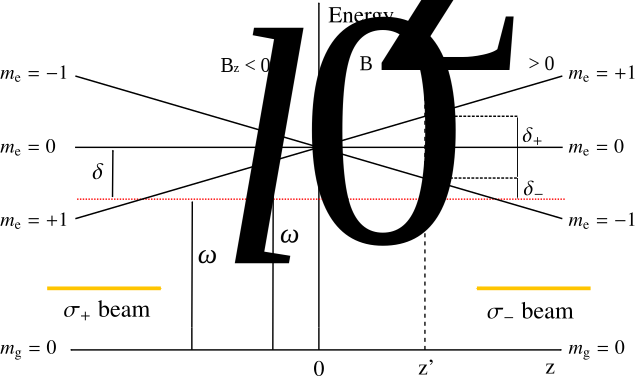
\includegraphics[width=0.9\columnwidth]{MOT_Energy.pdf}
%	\caption[Atomic scheme of energies inside the \ac{mot} for a $J=0 \rightarrow J'=1$ transition in the z axis]{Atomic scheme of energies inside the \ac{mot} for a $J=0 \rightarrow J'=1$ transition in the z axis. It shows the Zeeman splinting of the excited state with $J'=1$ into three different states with $m_e = -1, 0, 1$, due to the quadrupole magnetic field produced by two coils in anti-Helmholtz configuration. A counter-propagating pair of circularly polarized laser beams is represented by two yellow arrows. They have a frequency $\omega_l$ illustrated in the energetic scheme by a red dashed line. These optical beams are red-detuned by $\delta = \omega_0 - \omega_l$, where $\omega_0$ is the erbium frequency of the \SI{583}{\nano\meter} transition. Figure modified from original in \cite{Metcalf1999}.}\label{fig:MOT_Energy}
%\end{figure}


\subsection{\Acl{odt}}\label{subsec:Optical_dipole_trap}

As it has already been mentioned, the lowest possible temperature for the atoms trapped inside the \ac{mot} is just a few \si{\micro\kelvin}, which is not low enough to achieve the required critical temperature $T_C$ given by equation \eqref{eq:critical_temperature}. This prevents to form an erbium \acl{bec} with the use of only a \acl{mot}. Therefore, lower temperatures of the erbium ensemble must be reached by using an additional experimental phase known as \Acf{odt}. This type of trap is achieved with the use of a $\text{CO}_2$ laser beam at a wavelength of \SI{10.6}{\micro\meter} and a power of approximately \SI{60}{\watt}, which is focused in a focal point with \SI{25}{\micro\meter} of radius. This laser beam is aligned in a way that its focal point overlays with the region where atomic erbium is trapped inside the \ac{mot}. This way, the transference of atoms from \ac{mot} to \ac{odt} can be performed with the least possible losses in the total number of trapped atoms. 

In the different types of \acp{odt}, the one used here has the peculiarity that its $\text{CO}_2$ beam wavelength is far detuned for any erbium atomic transition. This type of \ac{odt} is commonly known as \Acf{quest} and were first proposed by T. Takekoshi et al. in 1994 \cite{Takekoshi1995}. Due to the far detuning between trap and atomic transitions, the trap can be approximated as a quasi-electrostatic field, which polarizes the atom and induces an atomic dipole moment \cite{Grimm2000}. The interaction between this induced dipole $\vec{p}$ and the electric field $\vec{E}(\vec{r})$ from the $\text{CO}_2$ laser, is described by an interaction potential $U_{\text{dip}}(\vec{r})$ given by
\begin{equation}\label{eq:interaction_potential}
	U_{\text{dip}}(\vec{r}) = -\frac{1}{2} <\vec{p} \cdot \vec{E}(\vec{r})>=-\frac{\text{Re}(\alpha) I(\vec{r})}{2 \epsilon_0 c},
\end{equation}
here, <> denotes time average over the rapid oscillating terms, $I(\vec{r}) = 2 \epsilon_0 c |\vec{E}(\vec{r})|^2$ is the laser intensity, and $\alpha$ the complex polarizability, such as $\vec{p} = \alpha(\omega_l) \cdot \vec{E}(\vec{r})$ with $\omega_l$ being the laser frequency. A good approximation can be obtained when considering the intensity distribution of the $\text{CO}_2$ laser beam as Gaussian:
\begin{equation}\label{eq:intensity_gaussian}
	I(\vec{r}, z) = \frac{2P}{\pi w^2(z)} e^{-2r^2/w^2(z)}.
\end{equation}
The distribution is represented in cylindrical coordinates with $z$ being the propagation direction and $\vec{r}$ the radial position. Additionally, $w(z)$ represents the beam radius and $P$ the optical power. Using now Equations \eqref{eq:interaction_potential} and \eqref{eq:intensity_gaussian}, the spatial behaviour of the interaction potential can be obtained as
\begin{equation}\label{eq:dipole_potential}
	U_{\text{dip}}(\vec{r}, z) =  -U_0 e^{-2r^2/w^2(z)},
\end{equation}
where $U_0 = \frac{\text{Re}(\alpha) P}{\epsilon_0 c \pi w_0^2}$ is the trap depth at the focal point of the trap beam (i.e. for $\vec{r} = 0$ and $z=0$), and $w_0=w(0)$ the beam waist at the focal point. Considering now, the atoms trapped inside the \ac{odt} with an energy lower than the maximal trap depth, the radial and longitudinal expansions would be considerably smaller than the trap scales i.e. the beam waist $w_0$ and Rayleigh length $z_R = \pi w_0^2/ \lambda$. This way, a Taylor expansion of $U_{\text{dip}}(\vec{r}, z)$  around the beam focal point can be performed
\begin{equation}\label{eq:harmonic_potential}
	U_{\text{dip}}(\vec{r}, z) \simeq  -U_0 \bigg[1-2\bigg(\frac{r}{w_0}\bigg)^2-\bigg(\frac{z}{z_R}\bigg)^2\bigg].
\end{equation}
This is equivalent to the expression for an harmonic oscillator inside a cylindrical potential. By using Equation \eqref{eq:harmonic_potential}, the generated dipole force $\vec{F}_{\text{dip}}$ affecting the neutral erbium atoms can be obtained as
\begin{equation}
	\vec{F}_{\text{dip}}(\vec{r}, z) = -\vec{\nabla}{U_{\text{dip}}(\vec{r}, z)}= -2U_0\bigg(\frac{2 r}{w_0^2}\hat{e}_r + \frac{z}{z_R^2}\hat{e}_z\bigg),
\end{equation}
where $\hat{e}_r$ is the radial and $\hat{e}_z$ the longitudinal unitary vectors in cylindrical coordinates. This final expression shows that for atoms close enough to the trap, there is a dipole force pushing them linearly towards its centre.

\subsection{Evaporative cooling}

Once atomic erbium is trapped in an \ac{odt}, the required temperatures for achieving a \ac{bec} can not yet be reached. During the \acl{odt} phase there is another cooling technique available, commonly known as Evaporative cooling, which allows for the reaching of temperatures lower than $T_C$ from Equation \eqref{eq:critical_temperature} \cite{Masuhara1988}. See Figure \ref{fig:evaporative_cooling}, the physical idea behind this phase is based on the fact that a group of trapped atoms have velocities, which follow a Maxwell-Boltzmann distribution with temperature $T_0$ and average velocity $\bar{v}$. Because of this, the temperature of a trapped atom ensemble, just requires letting the atoms with more energy leave the trap, while keeping the less energetic ones inside. This can be achieved by simply decreasing the laser intensity of the \ac{odt}'s beam, allowing for the atoms with higher energy to leave the trap. After this, the low energetic atoms inside the trap will interact via collisions with each other, restabilising the Maxwell-Boltzmann distribution and decreasing its temperature in a process called Re-thermalization. For a more effective cooling, this is performed in a continuous way and the speed at which the intensity is decreased becomes very important. Too fast would prevent the atoms from re-thermalizing and too slow would lead to problems with the maximum holding time of the trap. Any of both cases results in is inefficiency of the cooling process and the lost of too many atoms required to form a \ac{bec}. For more details on evaporative cooling refer to \cite{Ulitzsch2016, Metcalf1999, Roell2016}. The typical value reached for an erbium \ac{bec} are a number of around \num{30000}-\num{60000} atoms at temperature below \SI{200}{\nano\kelvin}.


\begin{figure}[!htbp]\centering
	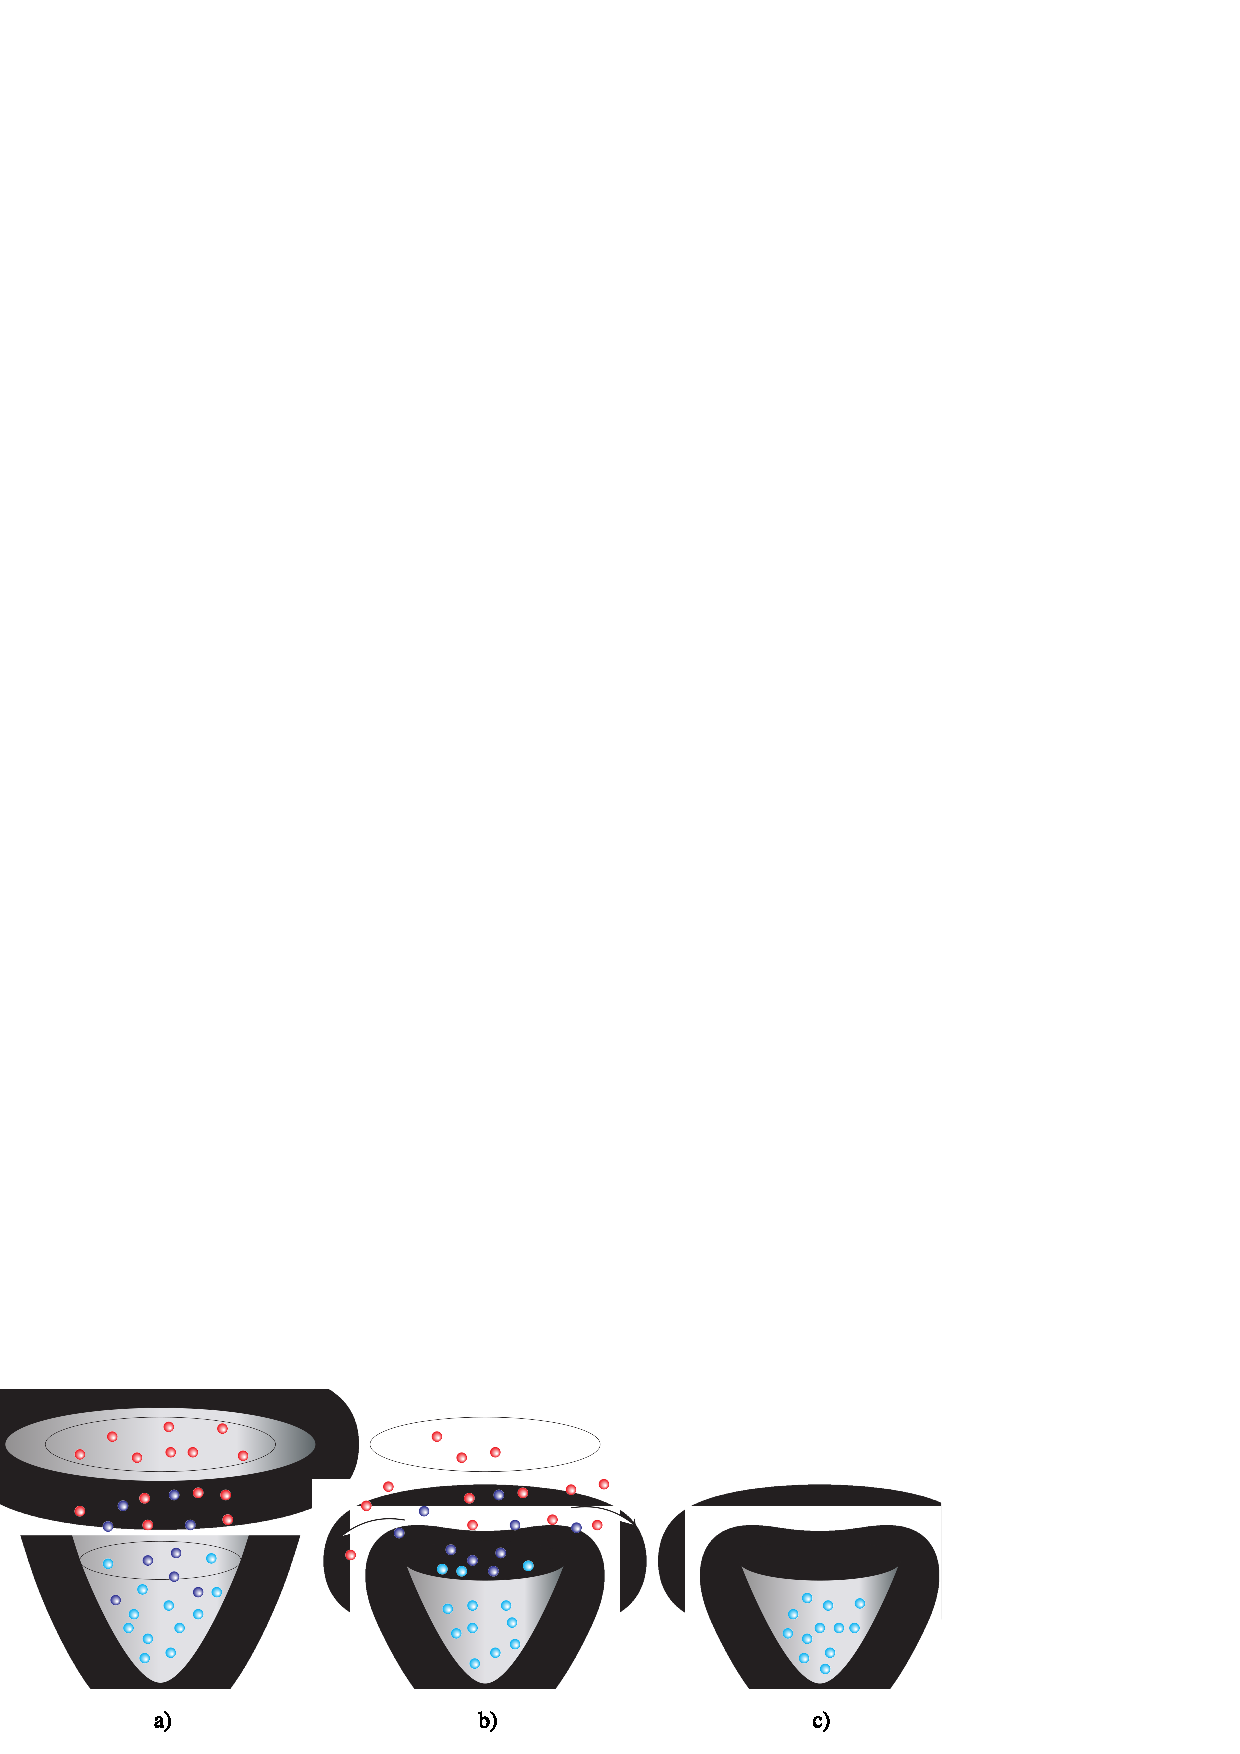
\includegraphics[width=1.\columnwidth]{evap_scheme.pdf}
	\caption[Evaporative cooling scheme]{Evaporative cooling scheme. A reduction in the beam intensity translates into a decrease of the potential. Thus, the more energetic atoms leave the trap and after some re-thermalization time, the average velocity of the system decreases causing a temperature drop. Figure taken from \cite{Rehberger2013}. }\label{fig:evaporative_cooling}
\end{figure}


\subsection{Absorption imaging}

Once an erbium \ac{bec} is obtained, it becomes necessary to have a process which allows to take images of the atomic cloud. This would allow to monitor the cloud behaviour along multiple experimental cycles, this phase is known as \Acf{ai} with its scheme shown in Figure \ref{fig:absorption_scheme}. To achieve this phase, first we turn off all the lasers and magnetic fields to shoot the atomic ensemble with a resonant light pulse of the near \SI{401}{\nano\meter} transition. As a result, the atoms would absorb the photons and re-emit them in all directions, reducing the intensity in different regions of the laser beam. This shadowed light beam is then received by a CCD camera, which takes an image. To obtain an optical density profile of the cloud, it is required to take two more images. The second one is taken a few \si{\milli\second} after the first, and receives the light from a second identical light pulse but once the atomic cloud is gone. Finally, the third one is taken without laser light entering the CCD sensor, and is simply used to quantify any background noise. This three images allow the calculation of a density profile $D(x,y)$ for any pixel located in the image with coordinates $x$ and $y$ by using the Beer-Lambert law \cite{Ulitzsch2016}.

\begin{equation}
	D(x,y)=-\text{ln}\bigg(\frac{I(x,y)-I_{D}(x,y)}{I_0(x,y)-I_D(x,y)}\bigg)
\end{equation}

Where $I(x,y)$ represents the light intensity measured in the pixel $(x,y)$ for the first image,  $I_0(x,y)$ intensity from the second image and $I_D(x,y)$ from the third image. From this density profile, multiple parameters of the cloud can estimated. One of those is the atom number, which can be obtained by integration of $D(x,y)$ and product with the inverted scattering cross-section of erbium. Other parameters are the position and radius of the atomic cloud, which allow relevant calculations such as the cloud temperature. For more information on this process, calculation of parameters or any procedure related with the formation of an erbium \ac{bec} refer to \cite{Ulitzsch2016, Roell2016}.

\vspace{1cm}

\begin{figure}[!htbp]\centering
	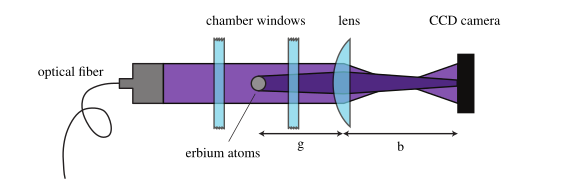
\includegraphics[width=1.\columnwidth]{absorption_scheme.pdf}
	\caption[Scheme of the absorption imaging process]{Scheme of the absorption imaging process. The atomic ensemble is illuminated with resonant light from the \SI{401}{\nano\meter} transition, and the shadow image is received by the CCD camera. After some few \si{\milli\second}, a second picture is taken with an exactly equal light pulse. And finally, a third picture is taken with no light pulse. These three images allow to generate a density image of the atomic cloud. Figure taken from \cite{Brammer2016}}\label{fig:absorption_scheme}
\end{figure}


%%% Local Variables: 
%%% mode: latex
%%% TeX-master: "Thesis"
%%% End: 
\include{3_thesis_bec_diffraction}
% !TEX root = Thesis.tex

%==============================================================================
\chapter{Towards Raman manipulation of spin-momentum state components}
\label{chap:raman_manipulation}
%==============================================================================



%%% Local Variables: 
%%% mode: latex
%%% TeX-master: "Thesis"
%%% End: 

% !TEX root = Thesis.tex

%==============================================================================
\chapter{Results and discussion}
\label{chap:results_and_discussion}
%==============================================================================

Once the theoretical description of the experiment has been completely introduced, the following part consist in the exposition of the obtained results together with a discussion concerning its correspondence with the announced theory. Due to this, the first step must be the Raman beams characterization with the measurement of each beam radius. This will allow in the next parts to make a direct correlation between beam power and intensity, which will be crucial for the whole experimental characterization.

\section{Measurement of the Raman beams radius}

These laser beams of the \SI{841}{\nano\meter} transition have been considered during all the theory as Gaussian beams. Therefore, they are described spatially by Equation \eqref{eq:intensity_gaussian}, which gives the relation between beam power $P$ and maximum intensity $I_{0}$ as
\begin{equation}
	I_0 = \frac{2P}{\pi w_0^2},
\end{equation}
where $w_0$ represents the beam radius at the atomic cloud position. Thus, a measurement of this quantity must be performed in order to obtain $I_0$ from the beam power. Figure \ref{fig:raman_beams_radius} shows both horizontal and vertical measurements for the two beams with the use of a knife-edge method. These data points were fit to an error function, which gave the estimations for $w_0$ in every case. From averaging the vertical and horizontal estimations of $w_0$ one gets the final measurement to be
\begin{align*}
	w_{01} &= (0.4961\pm0.0012)\si{\milli\meter}   &   w_{02} &= (0.8778\pm0.0024)\si{\milli\meter}.
\end{align*}
Note that the use of 1 and 2 for the Raman beams is also used as a distinction tool in Figure \ref{fig:raman_set_up}. As one can observe, the difference in beam size is approximately a factor of 3 between both beams. This must be compensated by adjusting the beam powers; however, it is a strong mismatch in the parameters that could not be solved due to time constraints. Therefore, the discussion part of the following measurements will have into account this mismatch in beam sizes as a source of possible non-correspondence between theory and experiment.

\pagebreak

\begin{figure}
	\centering
	\begin{subfigure}{.5\textwidth}
		\centering
		\includegraphics[width=1.\linewidth]{Fiber 1.pdf}
		\caption{Raman beam 1 (R1)}
		\label{fig:raman_beams_radius_1}
	\end{subfigure}%
	\begin{subfigure}{.5\textwidth}
		\centering
		\includegraphics[width=0.955\linewidth]{Fiber 2.pdf}
		\caption{Raman beam 2 (R2)}
		\label{fig:raman_beams_radius_2}
	\end{subfigure}
	\caption[Beam radius measurement of the Raman beams performed with a knife-edge method]{Beam radius measurement of the Raman beams performed with a knife-edge method. The beam profile was measured at approximately the atomic cloud position. Each of the beams were measured in a vertical (red) and horizontal (orange) position.}
	\label{fig:raman_beams_radius}
\end{figure}


\section{Characterization of the \SI{841}{\nano\meter} erbium transition with a \ac{bec}}

The following part consists in studying the \SI{841}{\nano\meter} erbium transition by blocking arbitrarily the beam R2 and allowing R1 to interact freely with the erbium \ac{bec}. This way, the Raman beam frequency can be locked in every cycle to a specific value. After an interaction time of 10\si{\milli\second} in the final part of the evaporation phase, the atomic ensemble falls freely during a \ac{tof} of 20\si{\milli\second}. Then, the measurement is taken with the absorption imaging phase. From these measurements, the number of atoms can be estimated and the result, after scanning the frequency of R1, is shown in Figure \ref{fig:resonance_841_transition}. The data with a maximum of $N_\text{max} = 34849$ atoms was taken as normalization factor. As it can be seen from the image, the plot shows a drop in the atom number when R1 is locked to a wavelength of approximately \SI{840.98827}{\nano\meter} in air. This is because most of the atoms forming a \ac{bec} are resonant at this wavelength and get excited by the R1 beam, which expel them out of the ensemble and reduce drastically the atom number. In order to avoid effects like power broadening, the optical power of R1 has been kept as low as possible: $P_{\text{R1}} = (49.0 \pm 0.5) \si{\milli\watt}$. This way, the Gaussian fit performed in Figure \ref{fig:resonance_841_transition} gives an estimation of the resonant wavelength $\lambda_0^*$ and the linewidth broadened mostly due to the beam power $\Delta\nu_{\text{PB}}$ as
\begin{align*}
	\lambda_0^* &= 840.988266(2)\si{\nano\meter}   &   \Delta\nu_{\text{PB}} &= (3600 \pm 1700)\si{\kilo\hertz}
\end{align*}

The result is a quite accurate estimation of $\lambda_0^*$ while the calculation for $\Delta\nu_{\text{PB}}$ is not. The main reason is due to limitations in the scanning precision of the wave-meter, which was locking the laser. In any case, the measurement of $\Delta\nu_{\text{PB}}$ is helpful when comparing it to the theoretical linewidth of the transition $\Delta\nu_0 = \Gamma/2\pi = \SI{7.96}{\kilo\hertz}$ (see Table \ref{tab:Transitions}). Giving a real scenario of how big the one-photon detuning $\delta$ must be to make reasonable the approximations used for the Raman transition processes. On the other hand, the estimation of $\lambda_0^*$ contains a source of errors that has not been considered so far. This is the uncertainty coming from the laser frequency lock, which can not be assumed to remain constant and may shift during measurements. For this reason, the one-photon detuning $\delta$ estimation will be obtained with by using as resonance wavelength in air the following value:
\begin{equation*}
	\lambda_{0} = 840.98827(1)\si{\nano\meter}
\end{equation*}

\begin{figure}\centering
	\includegraphics[width=1.\columnwidth]{Plot_resonance.pdf}
	\caption[Interaction of an erbium \ac{bec} with the beam R1]{Interaction of an erbium \ac{bec} with the beam R1. The plot shows the atom number of the \ac{bec}, normalized to the maximum measured value, as a function of the R1 wavelength in air. The interaction between R1 and the atomic ensemble lasts 10\si{\milli\second} before the end of evaporation phase in every experimental cycle. Each measured point has been obtained by averaging the atom number of 5 experimental cycles. }\label{fig:resonance_841_transition}
\end{figure}

\section{Diffraction of an erbium \ac{bec} with a 1D-lattice}

Now, it is the moment to study the diffraction of an erbium \ac{bec} with the described Raman lattice set-up. In order to do this, the one photon detuning $\delta$ must be measured. Due to the conclusions made in previous section, the optical frequency of the Raman beams has been chosen for this whole part to be $\lambda_\text{R} = 840.98880(1) \si{\nano\meter}$. Thus, the resulting value for $\delta$ turns out to be
\begin{equation*}
	\delta = 2\pi c\cdot\bigg(\frac{1}{\lambda_{0}} - \frac{1}{\lambda_\text{R}} \bigg) = 2\pi \cdot(225 \pm 6) \si{\mega\hertz} \approx \num{1.8e-5} \cdot\Delta\nu_0.
\end{equation*}

Therefore, the approximations used for the Hamiltonian in Section \ref{subsec:diffraction_regimes} are fulfilled. Because $\delta \gg \Gamma, \Delta\nu_0$ being the decay rate $\Gamma$ and natural linewidth $\Delta\nu_0$ of the \SI{841}{\nano\meter} transition (see Table \ref{tab:Transitions}). Another approximation that has been performed along this thesis results to be $\delta \gg \omega_r = \frac{\Delta_1}{4}$, with the 2-photon recoil frequency $\Delta_1$ given by Equation \eqref{eq:Bragg_condition} with $n=1$. From this expression one can get the value of $\Delta_1$ to be
\begin{equation*}
	\Delta_1 = \frac{2\hbar k^2}{M} = 2\pi \cdot (6.713 \pm 0.004)\si{kHz}.
\end{equation*}
This result proves the approximation $\delta \gg \Delta_1$ to also be reasonable within the described situation. Therefore, the different theoretical regimes seem to be valid and a more in-depth study is possible.

\subsection{Bragg regime}

As seen in Chapter \ref{chap:one_dimensional_lattices}, the Bragg regime is achieved only for long interaction times and when the Bragg condition is being fulfilled. To achieve it, the detuning between Raman beams has been set to $\Delta_1$. The result is an effective two level system between the 0th and +1st diffraction orders acting as ground and excited states respectively. This generates Rabi oscillations for different interaction times $t_\text{int}$ with frequency $\Omega_\text{eff}$ between the ground and excited state population rates, with the last one ideally governed by Equation \ref{eq:population_excited_state}. This effect has been observed for the case of optical power in the Raman beams chosen like: $P_1 = (3.05 \pm 0.05)\si{\milli\watt}$ and $P_2 = (9.10 \pm 0.05)\si{\milli\watt}$. These powers allow to estimate the ``effective'' intensity of the lattice as
\begin{equation*}
	I_\text{eff} = \sqrt{I_1\cdot I_2} = (7.7 \pm 0.4)\si{\kilo\watt\per\meter\squared}.
\end{equation*} 

Figure \ref{fig:Bragg_images} shows the effect of Rabi oscillations between the 0th and 1st orders for the exposed value of $I_\text{eff}$. These images are just a small sample of all the measured for this same situation but different values of $t_\text{int}$. From each image, the population rate of any $i$ order with $i \in \{0,1\}$ can be estimated as
\begin{equation}
	P_i = \frac{N_i}{N_0+N_1},
\end{equation}
where $N_0$ and $N_1$ are the number of atoms in each diffraction order. Therefore, it is possible to measure the population rate in each picture and plot it as a function of $t_\text{int}$. This is shown in Figure \ref{fig:Bragg_measurement}.

\begin{figure}[!htbp]
	\centering
	\begin{subfigure}{.33\textwidth}
		\centering
		\includegraphics[width=.9\linewidth]{Rabi_measurement_60us.png}
		\caption{ $t_\text{int} = 60\si{\micro\second}$}
		\label{fig:Bragg_images_1}
	\end{subfigure}%
	\begin{subfigure}{.33\textwidth}
		\centering
		\includegraphics[width=.9\linewidth]{Rabi_measurement_120us.png}
		\caption{ $t_\text{int} = 120\si{\micro\second}$}
		\label{fig:Bragg_images_2}
	\end{subfigure}
	\begin{subfigure}{.33\textwidth}
		\centering
		\includegraphics[width=0.9\linewidth]{Rabi_measurement_240us.png}
		\caption{ $t_\text{int} = 240\si{\micro\second}$}
		\label{fig:Bragg_images_3}
	\end{subfigure}
	\caption[Diffracted ultracold erbium ensemble after an interaction time with the lattice $t_\text{int}$ and a \ac{tof}$=19\si{\milli\second}$]{Diffracted ultracold erbium ensemble after an interaction time with the lattice $t_\text{int}$ and a \ac{tof}$=19\si{\milli\second}$. One can observe the effect of Rabi oscillations due to different $t_\text{int}$ values. The top atomic cloud corresponds to the 0th diffraction order while the bottom cloud is the 1st. Each image has been normalized with respect to the maximum and minimum value in the frame. The used camera is rotated 90° counter-clockwise, resulting in the separation of orders in the vertical axis of the frames. The effective intensity of the lattice used was $I_\text{eff} = (7.7 \pm 0.4)\si{\kilo\watt\per\meter\squared}$.}
	\label{fig:Bragg_images}
\end{figure}

\begin{figure}[!htbp]\centering
	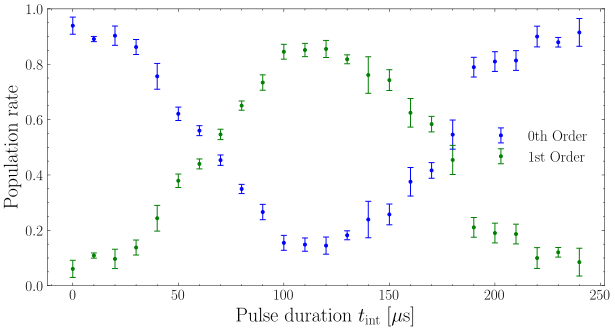
\includegraphics[width=1.\columnwidth]{Rabi_measurement_7.7.pdf}
	\caption[Population rate as a function of the interaction time between erbium \ac{bec} and Raman lattice]{Population rate as a function of the interaction time between erbium \ac{bec} and Raman lattice. The plot shows Rabi oscillations in rate populations of the 0th and 1st diffraction orders. Each pair of points has been taken by averaging 5 different images. The Raman lattice had an effective intensity of $I_\text{eff} = (7.7 \pm 0.4)\si{\kilo\watt\per\meter\squared}$. }\label{fig:Bragg_measurement}
\end{figure}

The plot confirms the theory and shows Rabi oscillations in an effective 2-level system as a predominant effect for this regime of parameters. Once this set of data is obtained, one can perform a more in-depth analysis of the oscillations. As it has been said, Equation \ref{eq:population_excited_state} must be fulfilled in this regime for the behaviour of population in the 1st diffracted order $P_1$. This way, a sine squared function fit can be performed to this population rate. However, in order to account for factors like noise or coherent losses in the \ac{bec}, a damped term has been added. Thus, the fitted function expression results
\begin{equation}
	f_\text{fit}(t_\text{int}) = A \text{exp}(-b t_\text{int}) \cdot \text{sin}^2\bigg(\frac{\Omega_\text{eff}t_\text{int}}{2} +\phi\bigg) + y_0,
\end{equation}
where $A$, $b$, $\Omega_\text{eff}$, $\phi$ and $y_0$ are free parameters of the fit. This allows the estimation of relevant system parameters such as the 2-photon Rabi frequency for any value of $I_\text{eff}$. The result can be seen in Figure \ref{fig:Bragg_fit_1st_order} for three different values of $I_\text{eff}$. From this analysis, one can easily see a proportional relation between $I_\text{eff}$ and $\Omega_\text{eff}$, which is also described in the theory. When combining Equations \eqref{eq:relation_rabi_frequency_lattice_depth} and \eqref{eq:relation_lattice_potential_depth_final} one gets
\begin{equation}\label{eq:relation_Ieff_omega_eff}
	\Omega_\text{eff} = \Bigg(\frac{3 \pi c^2 \Gamma}{\omega_0^3 \delta \hbar} \text{exp}\bigg(-\frac{r_1^2}{w_1^2}-\frac{r_2^2}{w_2^2}\bigg)\Bigg) \cdot I_\text{eff},
\end{equation}
which contains an exponential term describing how ``good'' the Raman beams are aligned with respect to the erbium \ac{bec}. Unfortunately, this term can not be measured independently within a reasonable value of uncertainty. However, it can be estimated with the obtained data by simply performing a linear fit to the measured values of $\Omega_\text{eff}$ as a function of $I_\text{eff}$. This can be seen in Figure \ref{fig:Linear_fit}.


\begin{figure}[!htbp]
	\centering
	\begin{subfigure}{1.\textwidth}
		\centering
		\label{fig:fig:Bragg_fit_1st_order_7.7}
		\includegraphics[width=.8\linewidth]{Rabi_fit_7.7.pdf}
		%\caption{$I_\text{eff} = (7.7\pm 0.4)\si{\kilo\watt\per\meter\squared}$}
	\end{subfigure}%
	\hfill
	\vspace{0.2cm}
	\begin{subfigure}{1.\textwidth}
		\centering
		\label{fig:Bragg_fit_1st_order_12.7}
		\includegraphics[width=.8\linewidth]{Rabi_fit_12.7.pdf}
		%\caption{$I_\text{eff} = (12.7\pm 0.4)\si{\kilo\watt\per\meter\squared}$}
	\end{subfigure}
	\hfill
	\vspace{0.2cm}
	\begin{subfigure}{1.\textwidth}
		\centering
		\label{fig:Bragg_fit_1st_order_24.6}
		\includegraphics[width=0.8\linewidth]{Rabi_fit_24.6.pdf}
		%\caption{$I_\text{eff} = (24.6\pm 0.4)\si{\kilo\watt\per\meter\squared}$}
	\end{subfigure}
	\caption[Fit of a damped sine squared function to the population rate for different values of $I_\text{eff}$]{Fit of a damped sine squared function to the population rate for different values of $I_\text{eff}$. The objective is to characterize the Rabi oscillations in this state and obtain an estimation of the 2-photon Rabi frequency $\Omega_\text{eff}$.}
	\label{fig:Bragg_fit_1st_order}
\end{figure}

\begin{figure}[!htbp]\centering
	\includegraphics[width=1.\columnwidth]{Linear_Fit.pdf}
	\caption[Linear fit of the 2-photon Rabi frequency as a function of the effective intensity in the lattice]{Linear fit of the 2-photon Rabi frequency as a function of the effective intensity in the lattice.}\label{fig:Linear_fit}
\end{figure}

\newpage

As a result, the linear fit seems to fulfil very accurately the measured data behaviour, which also coincides with theory. One could argue, the amount of data points to not be high enough. This is due to time constrains at the moment of taking the data, as different experimental problems appeared together with the requirement of measuring more data that will be shown below. In any case, the linear fit also shows a discrepancy with Equation \eqref{eq:relation_Ieff_omega_eff}, which consist in a non-zero intercept of $(2.97\pm0.05)\si{\kilo\hertz}$. This can be due to different reasons, the main one being the differences between Raman beam sizes. It could be a mayor factor because together with the beam misalignment, there will be a major difference between the optical intensities perceived by the \ac{bec}. This produces a shift in the lattice potential, which in principle should not affect these measurements for small shift values, but in the case of very big ones it could be a responsible factor. Other possibility is that the little amount of points covers a non-linear behaviour for small values of $I_\text{eff}$ for unknown reasons. In any case, the slope estimation of $(0.214\pm0.003)\si{\kilo\hertz\meter\squared\per\kilo\watt}$ allows the calculation of a ``misalignment'' factor $\beta$ as
\begin{equation*}
	\beta \equiv \text{exp}\bigg(-\frac{r_1^2}{w_1^2}-\frac{r_2^2}{w_2^2}\bigg) = (8.5\pm0.3)\cdot10^{-3},
\end{equation*}
which gives a maximum misalignment distance between the \ac{bec} position and R1/R2 beams' centre to be $r_1^\text{max} = (1.083 \pm 0.003) \si{\milli\meter}$ and  $r_2^\text{max} = (1.384\pm0.006) \si{\milli\meter}$ respectively. These values are within a reasonable order, but the alignment factor seems to be of very low quality for the implemented theoretical model.

\pagebreak

\subsection{Raman-Nath regime}

Once, the Bragg regime has been characterized, it is the moment of briefly showing that the Raman-Nath regime is also achievable in this experimental set-up. After ramping up the effective intensity in the optical lattice to $I_\text{eff} = (42.12 \pm 0.5)\si{\kilo\watt\per\meter\squared}$, and setting the 2-photon detuning between R1 and R2 to zero. The result can be seen in Figures \ref{fig:raman_nath} and \ref{fig:raman_nath_cut}, where an average of over 104 different pictures for a changing interaction time $t_\text{int} = 0\si{\micro\second}\text{ - }100\si{\micro\second}$ has been performed. As it can be seen, up to 5 different diffraction orders can be distinguished, which confirms the described theory and shows the experimental set-up capability to achieve the Raman-Nath regime.

\begin{figure}[!htbp]\centering
	\includegraphics[width=1.\columnwidth]{raman_nath.pdf}
	\caption[Absorption image of a multiple orders diffracted \ac{bec} after a \ac{tof} of \SI{19}{\milli\second}]{Absorption image of a multiple orders diffracted \ac{bec} after a \ac{tof} of \SI{19}{\milli\second}. The result was obtained after an average of over 104 different pictures with an effective intensity of $I_\text{eff} = (42.12 \pm 0.5)\si{\kilo\watt\per\meter\squared}$. The image has been rotated to match the gravitational axis with the up-down axis in the frame.}\label{fig:raman_nath_cut}\label{fig:raman_nath}
\end{figure}

\begin{figure}[!htbp]\centering
	\includegraphics[width=1.\columnwidth]{raman_nath_cut.pdf}
	\caption[Average cut performed to the image shown in Figure \ref{fig:raman_nath}]{Average cut performed to the image shown in Figure \ref{fig:raman_nath}}
\end{figure}

\pagebreak

\section{Magnetic fields characterization with \acs{rf} transitions}

After characterising an optical set-up that results in Raman transitions between components in the momentum space, the following goal is already described in Chapter \ref{chap:raman_manipulation}. This objective consists in obtaining Raman transitions between components in the spin and momentum space. But first, it is required the use of \ac{rf} transitions to estimate the Zeeman splitting caused by the magnetic fields inside the vacuum chamber. This way, the effect can be compensated first and then an extra field can be added along the quantization axis of the Raman beams, which will be required for the Raman transitions. Section \ref{sec:rf_transitions} describes this in further detail, while here the focus will be in analysing the measured data. Figure \ref{fig:RF_pulse} shows two reference samples of the measurements. An erbium \ac{bec} interacts with an \ac{rf}-pulse during \SI{0.4}{\milli\second} and falls through a gradient field of approximately 4G/cm during the \ac{tof} of \SI{19}{\milli\second}, which allows the separation between Zeeman states due to the Stern-Gerlach force. When the \ac{rf}-pulse frequency is far away from the Zeeman resonance $\omega_\text{Ze} \equiv \Delta E_{\text{Ze}}/\hbar$ given by Equation \ref{eq:Zeeman_splitting_difference}, the result is shown in Figure \ref{fig:RF_pulse_non-resonant}. The \ac{rf} transitions are being suppressed and the\ac{bec} remains mostly in the state $m_J=-6$ due to the experimental set-up configuration (see Section \ref{sec:rf_transitions}). On the other hand, when the \ac{rf}-pulse frequency is close to $\omega_\text{Ze}$, the transitions into other Zeeman levels are allowed, as shown in Figure \ref{fig:RF_pulse_resonant}. Therefore, by scanning the \ac{rf}-pulse frequency in the region of Zeeman resonance and comparing the population in different states, one can get an estimation of $\omega_\text{Ze}$ produced by any homogeneous magnetic field $\vec{B}_\text{H}$. Thus, the measurements of $\omega_\text{Ze}$ for three different homogeneous fields can be seen in Figure \ref{fig:Plot_RF_All_fields}.

\begin{figure}[!htbp]
	\centering
	\begin{subfigure}{.5\textwidth}
		\centering
		\includegraphics[width=1.\linewidth]{RF_pulse_non-resonant.pdf}
		\caption{Far-resonant \ac{rf} pulse}
		\label{fig:RF_pulse_non-resonant}
	\end{subfigure}%
	\begin{subfigure}{.5\textwidth}
		\centering
		\includegraphics[width=1.\linewidth]{RF_pulse_resonant.pdf}
		\caption{Near-resonant \ac{rf} pulse}
		\label{fig:RF_pulse_resonant}
	\end{subfigure}
	\caption[Comparative set of two different interactions between an erbium \ac{bec} and a \ac{rf}-pulse.]{Comparative set of two different interactions between an erbium \ac{bec} and a \ac{rf}-pulse. Both images were taken after an interaction time with the \ac{rf}-pulse of \SI{0.4}{\milli\second} and a \ac{tof} of \SI{19}{\milli\second}. During this \acl{tof} a gradient field of approximately 4G/cm was applied in order to separate the different $m_J$ orders. The gradient field direction was being applied along the gravitational axis, which corresponds to the left-right direction in both images.}
	\label{fig:RF_pulse}
\end{figure}



\begin{figure}[!htbp]
	\centering
	\begin{subfigure}{1.\textwidth}
		\centering
		\label{fig:Plot_RF_Experiment_fields}
		\includegraphics[width=.75\linewidth]{Plot_RF_Experiment_fields.pdf}
		\caption{Experiment magnetic field $\vec{B}_\text{H}$}
	\end{subfigure}%
	\hfill
	\begin{subfigure}{1.\textwidth}
		\centering
		\label{fig:Plot_RF_Compensated_fields}
		\includegraphics[width=.75\linewidth]{Plot_RF_Compensated_fields.pdf}
		\caption{Compensated magnetic field $\vec{B}_\text{Comp}$}
	\end{subfigure}
	\hfill
	\begin{subfigure}{1.\textwidth}
		\centering
		\label{fig:Plot_RF_Known_fields}
		\includegraphics[width=0.75\linewidth]{Plot_RF_Known_fields.pdf}
		\caption{Added magnetic field $\vec{B}'_\text{H} = \vec{B}_\text{Comp} +B_\text{R}\vec{e}_x$}
	\end{subfigure}
	\caption[Measured frequency spectrum of the \ac{rf} transitions for different homogeneous magnetic fields causing the splitting of Zeeman states in the erbium \ac{bec}]{Measured frequency spectrum of the \ac{rf} transitions for different homogeneous magnetic fields causing the splitting of Zeeman states in the erbium \ac{bec}. This data has been obtained measuring the population in each state and comparing the result for state $m_J = -6$ with the added population of the rest $m_J = $-5, -4, ..., +6. A Gaussian fit has been applied in each set of data in order to obtain an estimation of the resonant frequencies and transition linewidths.}
	\label{fig:Plot_RF_All_fields}
\end{figure}

\pagebreak

Each plotted data in the three parts of Figure \ref{fig:Plot_RF_All_fields} corresponds to a ratio of the atom number in the ground state $m_J = -6$ and the rest of states $m_J = $-5, -4, ..., +6. The different fields are: $\vec{B}_\text{H}$ the default magnetic field affecting the \ac{bec} during the experiment, $\vec{B}_\text{Comp}$ the compensated field with offset coils in order to make $\omega_\text{Ze}$ as low as possible, and $\vec{B}'_\text{H} = \vec{B}_\text{Comp} +B_\text{R}\vec{e}_x$ the result of adding to the compensated field and extra one in the quantization axis for the following section. By applying a Gaussian fit to each set of data, an estimation of relevant parameters like the Zeeman resonant frequencies $\omega_\text{Ze}$ and the \ac{rf} transition linewidths $\Delta \omega_\text{Ze}$ were obtained:

\begin{table}[htbp] \centering
	\begin{tabular}{@{}l|c|c@{}}\hline
	Magnetic field	                  & $\omega_\text{Ze} [\si{\kilo\hertz}]$           & $\Delta \omega_\text{Ze} [\si{\kilo\hertz}]$ \\ \hline\hline
	$\vec{B}_\text{H}$	     &  $588.1 \pm 0.1 $   & $1.1 \pm 0.4 $        \\
	$\vec{B}_\text{Comp}$	 &  $57.06 \pm 0.15 $  & $3.0 \pm 0.9 $        \\ 
	$\vec{B}'_\text{H}$	     &  $891.08 \pm 0.14 $ & $1.4 \pm 0.7 $       \\\hline
	\end{tabular}
	\caption[Estimation of the Zeeman resonant frequencies $\omega_\text{Ze}$ and the \ac{rf} transition linewidths $\Delta \omega_\text{Ze}$]{Estimation of the Zeeman resonant frequencies $\omega_\text{Ze}$ and the \ac{rf} transition linewidths $\Delta \omega_\text{Ze}$ from the Gaussian fits performed in Figure \ref{fig:Plot_RF_All_fields}.}
	\label{tab:results_Plot_RF_All_fields}
\end{table}

These results are within expectation and for the case of $\Delta \omega_\text{Ze}$ show of stable are the Zeeman splitting and magnetic field. As a result, one can conclude for the next section that the Raman condition for the 2-photon detuning $\Delta$ must be of approximately $890\si{\kilo\hertz}$ with an error margin of $58\si{\kilo\hertz}$ given by $\omega_\text{Ze}$ for the compensated fields.

\section{Raman transitions in the spin-momentum space}

Finally, the last measurement achieved in this thesis correspond to Raman transitions between Zeeman states. In order to achieve it, the offset coils of the experiment have been configured to produce the magnetic field $\vec{B}'_\text{H}$, which is mostly pointing throughout the Raman beams axis. After this, the Raman beams were re-aligned and their radius at the \ac{bec} position reduced to:
\begin{align*}
	w_{01} &= (66.9\pm1.5)\si{\micro\meter}   &   w_{02} &= (71.1\pm 1.1)\si{\micro\meter}
\end{align*}

Moreover, the beams polarization was changed from linear to circular, in order to achieve the experimental set-up described in Section \ref{sec:raman_manipulation_theory}. The optical powers for each beam were approximately $50\si{\milli\watt}$. And, the 2-photon detuning between beams was adjusted by using the value obtained at the previous section and Equation \eqref{eq:raman_condition} as $\Delta_\text{R} \approx 2\cdot840 \si{\kilo\hertz}$. There result was the obtention of Raman transitions in the spin-momentum space, which can be seen in Figure \ref{fig:raman_gradient}. For both cases, the images were taken after an interaction time with the Raman beams and a \ac{tof} of \SI{220}{\micro\second} and \SI{20}{\milli\second} respectively. The only difference between both images is that Figure \ref{fig:raman_without_gradient} had no gradient field being applied during the \ac{tof} and \ref{fig:raman_with_gradient} did have it of roughly 4G \si{\per\centi\meter}. The result is that the orders generated in the first image do not suffer an Stern-Gerlach force, described by Equation \ref{eq:Stern-Gerlach_force}, while the second image does suffer from this effect. Due to this, the Raman orders are separated in the gradient direction as a function of their spin value $m_J$, apart from the separation due to different momentum transfer that remains the unaltered. This effect proves without a doubt the internal energetic difference between orders and the achievement of Raman transitions in states with different spin. After this, an in-depth study of the experimental system would be required. However, time constraints during the realization of this thesis will leave this achievement aside for a future work.

\begin{figure}[!htbp]
	\centering
	\begin{subfigure}{.5\textwidth}
		\centering
		\includegraphics[width=0.7\linewidth]{raman_without_gradient.pdf}
		\caption{Without magnetic gradient}
		\label{fig:raman_without_gradient}
	\end{subfigure}%
	\begin{subfigure}{.5\textwidth}
		\centering
		\includegraphics[width=0.7\linewidth]{raman_with_gradient.pdf}
		\caption{With magnetic gradient}
		\label{fig:raman_with_gradient}
	\end{subfigure}
	\caption[Comparative picture of Raman transitions between spin-momentum orders with and without gradient field interaction]{Comparative picture of Raman transitions between spin-momentum orders with and without gradient field interaction. This gravitational direction is again matched with the gradient field and corresponds to the left-right axis on both frames. In (b), the Stern-Gerlach force separates the diffracted orders as a function of the spin value $m_J$ throughout the gradient field direction. Proving the internal energy difference in each order. }
	\label{fig:raman_gradient}
\end{figure}

%%% Local Variables: 
%%% mode: latex
%%% TeX-master: "Thesis"
%%% End: 


% Uncomment the following command to get references per chapter.
% Put it inside the file or change \include to \input if you do not want the references
% on a separate page
% \printbibliography[heading=subbibliography]

%------------------------------------------------------------------------------
% Use biblatex for the bibliography
% Add bibliography to Table of Contents
% Comment out this command if your references are printed for each chapter.
\printbibliography[heading=bibintoc]

%------------------------------------------------------------------------------
% Include the following lines and comment out \printbibliography if
% you use BiBTeX for the bibliography.
% If you use biblatex package the files should be specified in the preamble.
% \KOMAoptions{toc=bibliography}
% {\raggedright
%   \bibliographystyle{../Template/refs/atlasBibStyleWithTitle.bst}
%   % \bibliographystyle{unsrt}
%   \bibliography{./thesis_refs,../Template/refs/standard_refs-bibtex}
% }

%------------------------------------------------------------------------------
\appendix
% \part*{Appendix}
% Add your appendices here - don't forget to also add them to \includeonly above
\include{thesis_appendix}
% \printbibliography[heading=subbibliography]

%------------------------------------------------------------------------------
% Declare lists of figures and tables and acknowledgements as backmatter
% Chapter/section numbers are turned off
\backmatter

\listoffigures
\listoftables

%------------------------------------------------------------------------------
% Print list of acronyms
\printacronyms

%------------------------------------------------------------------------------
% You could instead add your acknowledgements here - don't forget to
% also add them to \includeonly above
% %------------------------------------------------------------------------------
\chapter*{Acknowledgements}
\label{sec:ack}
%------------------------------------------------------------------------------


%%% Local Variables: 
%%% mode: latex
%%% TeX-master: "../Template/Thesis"
%%% End: 


%------------------------------------------------------------------------------
% CV needed when you submit your PhD thesis
% \input{thesis_cv}

\end{document}

%%% Local Variables:
%%% mode: latex
%%% TeX-master: t
%%% End:
